\chapter{抽样调查基本概念}

\section{抽样调查的目的}
抽样调查最直接的主要任务,就是根据测得的样本(样本需要能够反应总体的差异)数量指标$\{y_1,y_2,\dots,y_n\}$,对总体$\{Y_1,Y_2,\dots,Y_N\}$的一些数字特征进行估计。如估计:
\begin{enumerate}
	\item $\text{总体均值}\mu=\frac{1}{N}\sum_{i=1}^NY_i,\;\text{总体总量}\tau=\sum_{i=1}^NY_i$。
	\item \footnote{这里指的是有限总体的方差,我们在抽样调查中认为有限总体也相当于一个样本,以样本方差公式计算其方差。在无限总体的情况下,分母取$N$。}$\text{总体方差}\sigma^2=\frac{1}{N-1}\sum_{i=1}^N(Y_i-\mu)^2$。
	\item 总体中满足某一特征的单元所占比例$p$。
	\item 总体分布的分位数。
\end{enumerate}

\section{目标群体、源群体、研究群体}
\begin{itemize}
	\item 目标群体:研究者希望对其进行描述或推断的群体。
	\item 源群体:研究者实际用于选择样本的群体,通常是目标群体的一个子集或一个接近目标群体的群体。
	\item 研究群体:抽样后的样本
\end{itemize}
\begin{figure}[htbp] 
	\centering 
	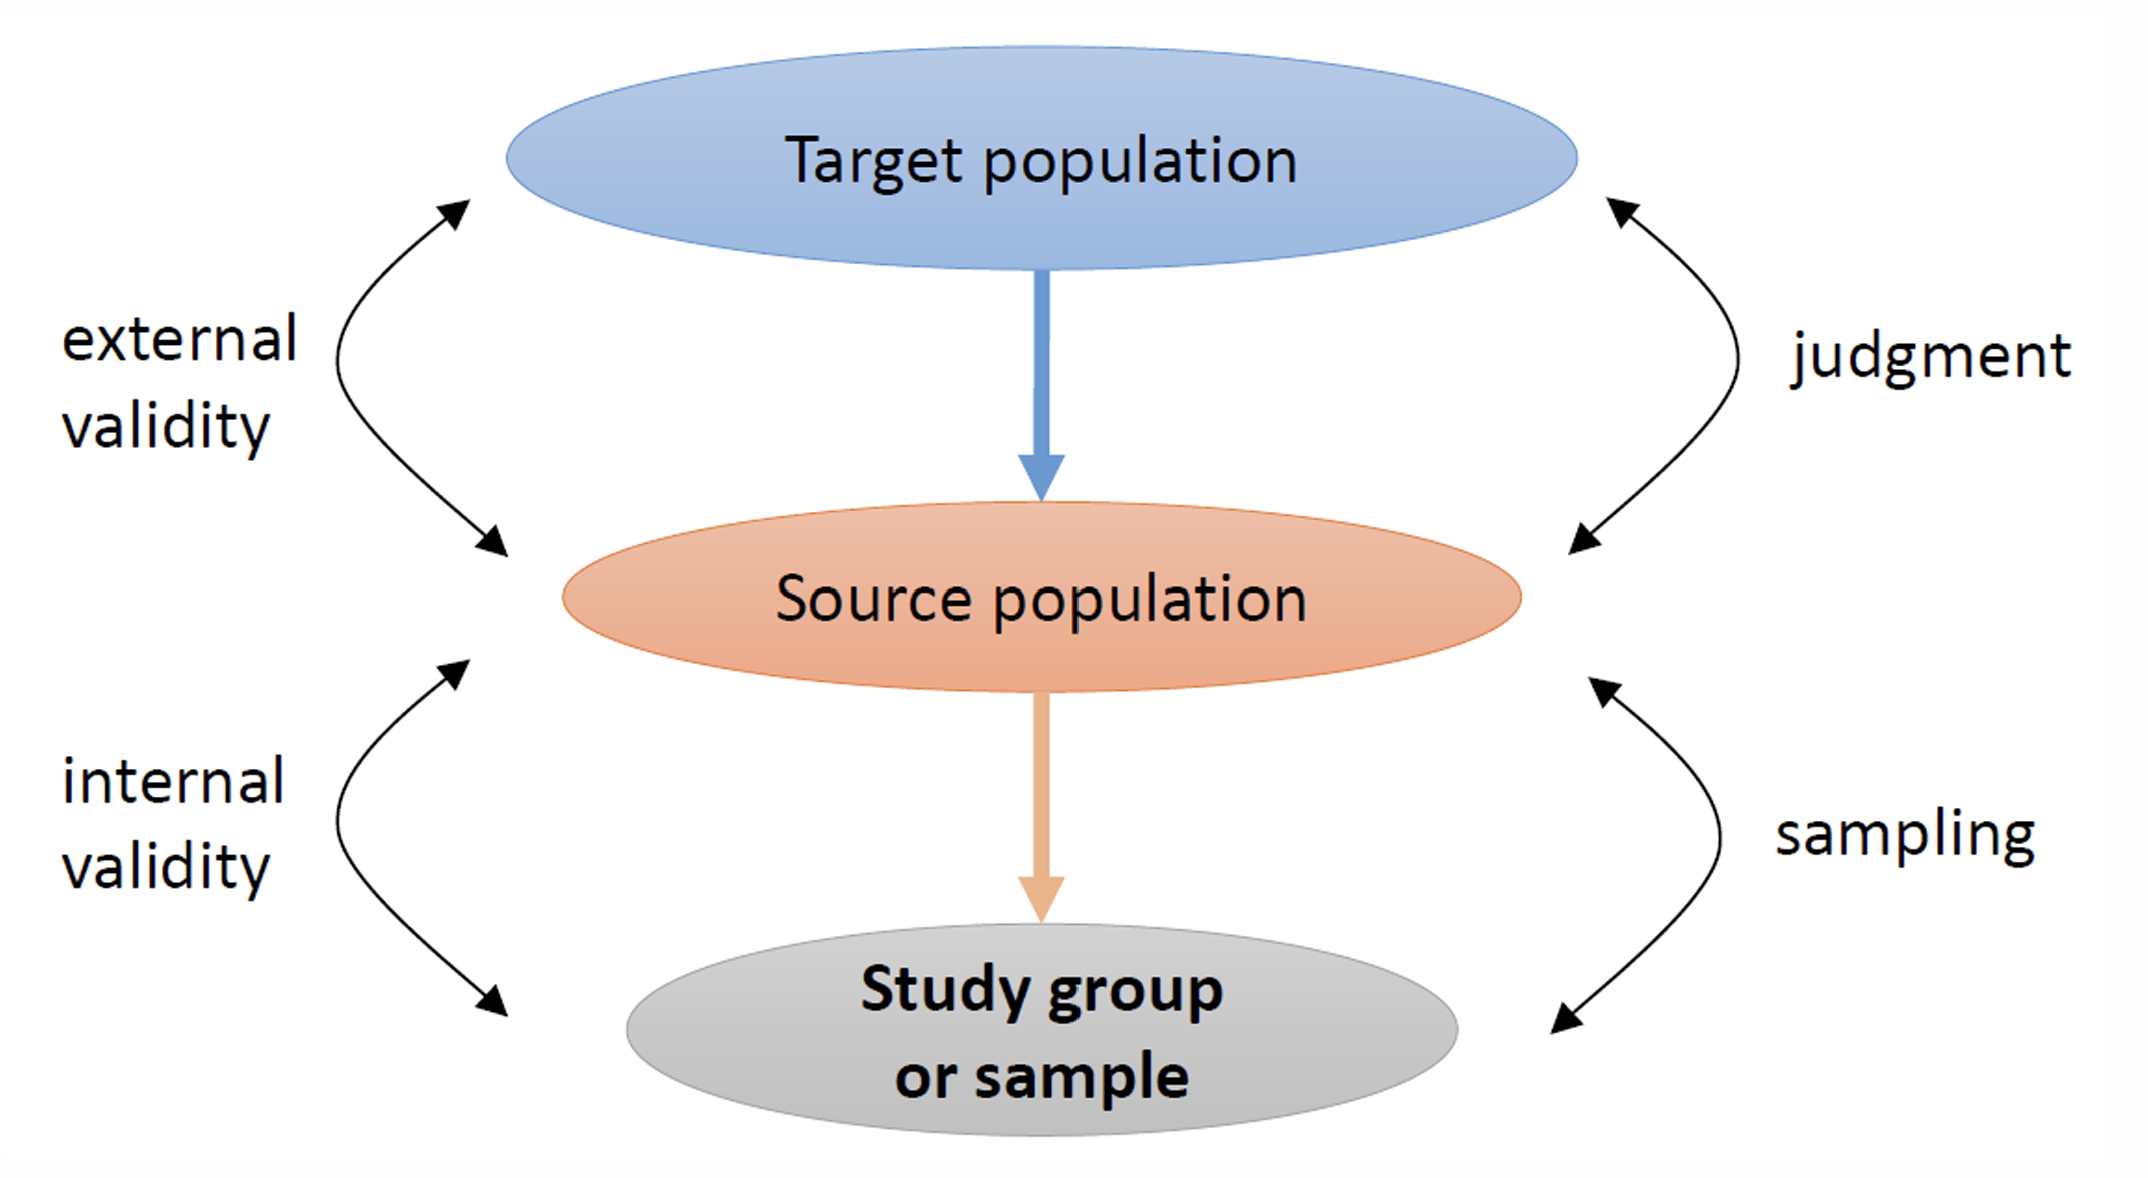
\includegraphics[width=0.8\textwidth]{sampling-method/introduction/population.png}
	\caption{群体} 
\end{figure}

\section{抽样设计}
\begin{center}
	\begin{equation}
		\text{抽样设计}
		\begin{cases}
			\text{概率抽样} 
			\begin{cases}
				\text{简单随机抽样} \\
				\text{分层抽样} \\
				\text{整群抽样} \\
			\end{cases}\\
			\text{非概率抽样}
			\begin{cases}
				\text{方便抽样} \\
				\text{雪球抽样} \\
				\text{判断抽样} \\
			\end{cases}
		\end{cases}\notag
	\end{equation}
\end{center}
\begin{itemize}
	\item 概率抽样样本是随机产生的,非概率抽样样本不是随机产生的。
	\item 非概率抽样无法判断样本是否具备代表性,也就无法确定抽样误差。但在一定程度上可以说明总体的特征。
	\item 方便抽样是选择最容易获得的样本作为研究对象。
	\item 雪球抽样是先选择一个较小的样本,再让这个样本中的样本单元去提供一些样本。
	\item 判断抽样是研究人员从总体中选择自己认为最能代表总体的个体作为样本。
\end{itemize}

\section{抽样框架}
对可以选择作为样本单元的群体单位列出的名册或排序编号,用以确定总体的抽样范围和结构。

\section{抽样调查随机性的来源}
\subsection{基于模型的方法}
绝大多数统计学课程是基于模型的(model-based approch),它将总体看作是背后随机变量的实现,随机性来源于随机变量的取值。
\subsection{基于设计的方法}
抽样调查是基于设计的(design-based approch),它将总体中个体的值看作为定值,而随机性来源于是否抽到该个体。

\section{概率抽样概述}
\subsection{样本概率}
记一个可能的样本为$s$,记在抽样设计下出现这个样本的概率\footnote{样本出现的概率未必是等可能的。}为$p(s)$,应有$\sum\limits_{s}p(s)=1$。
\subsection{入样概率与抽样权重}
对于任意个体$Y_k$,该个体的入样概率$\pi_k$记为$\sum\limits_{Y_k\in s}p(s)$,该个体的抽样权重$w_k$定义为$\frac{1}{\pi_k}$,表示该个体可以代表总体里的多少个个体。若每个个体的抽样权重都一样,则称产生的样本为\gls{SelfWeighting}样本。
